\documentclass[a4paper,11pt]{book}
\usepackage{listings}
\usepackage[utf8]{inputenc}
\usepackage[spanish,es-tabla]{babel}
\usepackage{pdflscape}
 
%\usepackage[style=list,number=none]{glossary}
\usepackage{titlesec}
%\usepackage{pailatino}

\decimalpoint
\usepackage{dcolumn}
\newcolumntype{.}{D{.}{\esperiod}{-1}}
\makeatletter
\addto\shorthandsspanish{\let\esperiod\es@period@code}
\makeatother

%\RequirePackage{verbatim}
%\RequirePackage[Glenn]{fncychap}
\usepackage{fancyhdr}
\usepackage{graphicx}
\usepackage{afterpage}
\usepackage{longtable}
\usepackage[pdfborder={000}]{hyperref} %referencia

% ********************************************************************
% Información reutilizable
% ********************************************************************
\newcommand{\asunto}{Trabajo de Fin de Grado}
\newcommand{\titulo}{Un portal de transparencia para datos libres}
\newcommand{\tituloEng}{A transparency portal for open data}
\newcommand{\titulacion}{Grado en Ingeniería Informática}
\newcommand{\autor}{Germán Martínez Maldonado}
\newcommand{\email}{germaaan@gmail.com}
\newcommand{\tutor}{Juan Julián Merelo Guervós}
\newcommand{\escuela}{Escuela Técnica Superior de Ingenierías Informática y de Telecomunicación}
\newcommand{\universidad}{Universidad de Granada}
\newcommand{\ciudad}{Granada}
\newcommand{\version}{Version 0.1}

\hypersetup{
pdfauthor = {\autor\ (\email)},
pdftitle = {\titulo},
pdfsubject = {\asunto},
pdfkeywords = {software libre, transparencia, datos abiertos, sistema de control de versiones, aprovisionamiento, tests, 
integración continua, despliegue automático},
pdfcreator = {LaTeX con el paquete texlive},
pdfproducer = {pdflatex}
}

%\hyphenation{}

\usepackage{url}
\usepackage{colortbl,longtable}
\usepackage[stable]{footmisc}
%\usepackage{index}

%\makeindex
%\usepackage[style=long,cols=2,border=plain,toc=true,number=none]{glossary}
%\makeglossary

% Redefinición de comandos
%\renewcommand{\indexname}{Índice alfabético}
%\renewcommand{\glossaryname}{Glosario}

\pagestyle{fancy}
\fancyhf{}
\fancyhead[LO]{\leftmark}
\fancyhead[RE]{\rightmark}
\fancyhead[RO,LE]{\textbf{\thepage}}
\renewcommand{\chaptermark}[1]{\markboth{\textbf{#1}}{}}
\renewcommand{\sectionmark}[1]{\markright{\textbf{\thesection. #1}}}

\setlength{\headheight}{1.5\headheight}

\newcommand{\HRule}{\rule{\linewidth}{0.5mm}}
%Definimos los tipos ejemplo y definición podremos usar estos tipos
\newtheorem{ejemplo}{Ejemplo}[chapter]
\newtheorem{definicion}{Definición}[chapter]

\definecolor{gray97}{gray}{.97}
\definecolor{gray75}{gray}{.75}
\definecolor{gray45}{gray}{.45}
\definecolor{gray30}{gray}{.94}

\lstset{
  frame=Ltb,
  framerule=0.5pt,
  aboveskip=0.5cm,
  framextopmargin=3pt,
  framexbottommargin=3pt,
  framexleftmargin=0.1cm,
  framesep=0pt,
  rulesep=.4pt,
  backgroundcolor=\color{gray97},
  rulesepcolor=\color{black},
  %
  stringstyle=\ttfamily,
  showstringspaces = false,
  basicstyle=\scriptsize\ttfamily,
  commentstyle=\color{gray45},
  keywordstyle=\bfseries,
  %
  numbers=left,
  numbersep=6pt,
  numberstyle=\tiny,
  numberfirstline = false,
  breaklines=true,
}
 
% Minimizar fragmentado de listados
\lstnewenvironment{listing}[1][]
  {\lstset{#1}\pagebreak[0]}{\pagebreak[0]}

% http://tex.stackexchange.com/questions/89574/language-option-supported-in-listings
\lstdefinelanguage{JavaScript}{
  keywords={typeof,new,true,false,catch,function,return,null,catch,switch,var,if,in,while,do,else,case,break},
  keywordstyle=\color{blue}\bfseries,
  ndkeywords={class,export,boolean,throw,implements,import,this},
  ndkeywordstyle=\color{darkgray}\bfseries,
  identifierstyle=\color{black},
  sensitive=false,
  comment=[l]{//},
  morecomment=[s]{/*}{*/},
  commentstyle=\color{purple}\ttfamily,
  stringstyle=\color{red}\ttfamily,
  morestring=[b]',
  morestring=[b]"
}

\lstdefinestyle{Consola}{
  basicstyle=\scriptsize\bf\ttfamily,
  backgroundcolor=\color{gray30},
  frame=single,
  numbers=none
}

\newcommand{\bigrule}{\titlerule[0.5mm]}

% Para que las páginas en blanco no tengan cabecera
\makeatletter
\def\clearpage{%
  \ifvmode
    \ifnum \@dbltopnum =\m@ne
      \ifdim \pagetotal <\topskip
        \hbox{}
      \fi
    \fi
  \fi
  \newpage
  \thispagestyle{empty}
  \write\m@ne{}
  \vbox{}
  \penalty -\@Mi
}
\makeatother

\usepackage{pdfpages}

\begin{document}
\begin{titlepage}

\newlength{\centeroffset}
\setlength{\centeroffset}{-0.5\oddsidemargin}
\addtolength{\centeroffset}{0.5\evensidemargin}
\thispagestyle{empty}

\noindent\hspace*{\centeroffset}\begin{minipage}{\textwidth}

\centering

\includegraphics[width=0.9\textwidth]{imagenes/logo_ugr.jpg}\\[1.4cm]

\textsc{\Large\asunto\\[0.2cm]}
\textsc{\titulacion}\\[1cm]

{\Huge\bfseries \titulo\\}
\noindent\rule[-1ex]{\textwidth}{3pt}\\[3.5ex]
\end{minipage}

\vspace{2.5cm}
\noindent\hspace*{\centeroffset}\begin{minipage}{\textwidth}
\centering

\textbf{Autor}\\ {\autor}\\[2.5ex]
\textbf{Tutor}\\ {\tutor}\\[2cm]

\includegraphics[width=0.3\textwidth]{imagenes/etsiit_logo.png}\\[0.1cm]
\textsc{\escuela}\\
\textsc{---}\\
\ciudad, \today
\end{minipage}
\end{titlepage}
\frontmatter

\begingroup
\let\cleardoublepage\clearpage
  \pagestyle{empty}
  \chapter*{}
%\thispagestyle{empty}
%\cleardoublepage

%\thispagestyle{empty}

%\cleardoublepage
%\thispagestyle{empty}

\begin{center}
{\large\bfseries \titulo}\\
\end{center}
\begin{center}
\autor\
\end{center}

\noindent{\textbf{Palabras clave}: software libre, transparencia, datos abiertos, sistema de control de versiones, 
aprovisionamiento, tests, integración continua, despliegue automático\\

\vspace{0.7cm}
\noindent{\textbf{Resumen}}\\

Desarrollar una plataforma para la transparencia y publicación de datos abiertos que sea desplegable en un infraestructura 
física o virtual basándose en el trabajo realizado en el portal UGR Transparente. Este desarrollo tendrá como objetivo que 
el resultado sea una plataforma totalmente basada en el software libre que se pudiera adaptar con facilidad a otro organismo, 
teniendo en cuenta funcionalidades y requisitos obligatorios, además de aspectos de accesibilidad y escalabilidad. 

\medskip
La herramientas básicas a usar serán un sistema de control de versiones y una plataforma de desarrollo colaborativo que 
albergue el proyecto, además usando dicho sistema de control de versiones. También se quiere que la plataforma se pueda ir 
desarrollando y administrando a la vez, por lo que para convertir todo esto es un proceso más ágil e ininterrumpido se usarán 
otras herramientas que permitan lo siguiente:

\begin{itemize}
  \item Realizar aprovisionamiento de las infraestructuras.
  \item Validación mediante tests unitarios.
  \item Comprobación de conflictos mediante integración continua.
  \item Actualizaciones mediante despliegue automático.
\end{itemize}

\cleardoublepage

\thispagestyle{empty}

\begin{center}
{\large\bfseries \tituloEng}\\
\end{center}
\begin{center}
\autor\\
\end{center}

%\vspace{0.7cm}
\noindent{\textbf{Keywords}: free software, transparency, opendata, version control system, provisioning, tests, continuous 
integration, automated deployment}\\

\vspace{0.7cm}
\noindent{\textbf{Abstract}}\\

Write here the abstract in English.

\chapter*{}
\thispagestyle{empty}

\noindent\rule[-1ex]{\textwidth}{2pt}\\[4.5ex]

Yo, \textbf{\autor}, alumno de la titulación \titulacion de la \textbf{\escuela\ de la \universidad}, con DNI XXXXXXXXX, 
autorizo la ubicación de la siguiente copia de mi Trabajo Fin de Grado en la biblioteca del centro para que pueda ser
consultada por las personas que lo deseen.

\vspace{6cm}

\noindent Fdo: \autor

\vspace{2cm}

\begin{flushright}
\ciudad, a \today
\end{flushright}

\chapter*{}
\thispagestyle{empty}

\noindent\rule[-1ex]{\textwidth}{2pt}\\[4.5ex]

D. \textbf{\tutor}, Profesor del Área de XXXX del Departamento de Arquitectura y Tecnología de Computadores de la \universidad.

\vspace{0.5cm}

\vspace{0.5cm}

\textbf{Informa:}

\vspace{0.5cm}

Que el presente trabajo, titulado \textit{\textbf{\titulo}}, ha sido realizado bajo su supervisión por \textbf{\autor}, y 
autorizo la defensa de dicho trabajo ante el tribunal que corresponda.

\vspace{0.5cm}

Y para que conste, expide y firma el presente informe en \ciudad\ a \today.

\vspace{1cm}

\textbf{El tutor:}

\vspace{5cm}

\noindent \textbf{\tutor}

\chapter*{Agradecimientos}
\thispagestyle{empty}

\vspace{1cm}

Poner aquí agradecimientos...



  \newpage
  \thispagestyle{empty}
  \
  
  \tableofcontents
  \listoffigures
  \listoftables
\endgroup

  \newpage
  \thispagestyle{empty}
  \
  \mainmatter
  \chapter{Introducción}

La transparencia en los organismos públicos es importante.

Los desarrollos de software con despliegue continuo son interesantes.
  \chapter{Objetivos}

El objetivo de este proyecto es el de obtener un portal de transparencia para la Universidad de Granada basado en el software 
libre que además permita una metodología de desarrollo en el que continuamente se puedan añadir nuevas funcionalidades a la 
vez que se van testeando, para después de una fácil integración culminar con un despliegue automático. Este portal no almacenará
los propios datos abiertos, si no que hará de presentación de los datos que estarán contenidos en otra plataforma destinada 
únicamente a dicho fin (OpenData UGR).

\bigskip
Un resumen de los principales objetivos a alcanzar son:

\begin{itemize}
  \item \textbf{OBJ-1.} Promover la idea de que los desarrollos bajo software libre en general y en la administración pública 
  en particular ayudan a generar confianza y demuestran compromiso con la transparencia.
  \item \textbf{OBJ-2.} Solucionar los problemas de generación de las tablas con los elementos de información.
  \item \textbf{OBJ-3.} Implementar en el portal UGR Transparente una metodología de desarrollo continuo que se base 
  en el uso de tests unitarios para cada una de las funcionalidades que se vayan añadiendo, test de 
  cobertura que evalúen los test unitarios, integración continua ante cambios introducidos, despliegue automático de las
  actualizaciones que se vayan produciendo y aprovisionamiento software para la infraestructura.
\end{itemize}

Además como objetivo secundario tendremos:

\begin{itemize}
  \item \textbf{OBJ-4.} Estudiar la posibilidad de hacer una instalación totalmente personalizada del portal de datos de código
  abierto CKAN para los datos abiertos de la Universidad de Granada, además de un aprovisionamiento que permitiera que esta 
  instalación se pudiera realizar automáticamente en una infraestructura.
\end{itemize}

\bigskip
Destacar en los aspectos formativos previos más utilizados para el desarrollo del proyectolos conocimientos sobre 
infraestructuras virtuales para el tema de gestión de configuraciones, ingeniería de software para el análisis del proyecto 
e ingeniería de servidores para la realización de pruebas desde el aspecto hardware.

\section{Alcance de los objetivos}

La aplicación resultante visualmente será idéntica que la versión actual de UGR Transparente, pero internamente habrá cambiado
totalmente la metodología de desarrollo, pasando de un desarrollo sin control a uno totalmente controlado mediante pruebas 
unitarias e integración continua. Además los cambios ya no se tendrá que aplicar manualmente en el servidor, sino que se hará
uso de un despliegue automático para tal fin.

\bigskip
Esta aplicación se usará de base en la Universidad de Granada, pero además el objetivo del desarrollo es que se pueda exportar 
para su uso en cualquier organización sin demasiada dificultad, de ahí que se vaya a estudiar también la posibilidad de 
personalización de CKAN, ya que esto permitiría generar una gran plataforma de liberación de datos totalmente personalizable
según el ámbito y las necesidades.

\section{Interdependencia de los objetivos}

Todos los objetivos son independientes entre sí, pero el primer objetivo (\textbf{OBJ-1}) es el principal motivador de este 
proyecto, por lo que aún sin representar el desarrollo de ningún trabajo en concreto es el que va a escudar y avalar el 
desarrollo de los otros. En aspectos más relacionados con la realización del proyecto, el segundo objetivo (\textbf{OBJ-2}) es
el que se solucionará de forma inmediata ya que impide el correcto funcionamiento del portal. El resto de objetivos serán 
tratados en mayor medida durante los capítulos de implementación y pruebas.


  \chapter{Planificación}

\section{Fases y entregas}

\subsection{Fases}

Como este va a ser un proyecto que ya cuenta con un trabajo previo realizado, la fase inicial de gestión va a ser muy breve
porque se parte de que ya se han realizado varias reuniones y el proyecto está parcialmente funcionando, por lo que no se parte
de cero, es una ampliación de un proyecto inicial.

\begin{itemize}
  \item \textbf{Fase 1:} Especificaciones del proyecto
  \item \textbf{Fase 2:} Planificación
  \item \textbf{Fase 3:} Análisis y diseño
  \item \textbf{Fase 4:} Implementación
  \item \textbf{Fase 5:} Pruebas
  \item \textbf{Fase 6:} Documentación
\end{itemize}

\subsection{Lista de entregas}

Se harán una serie de breves informes sobre el contenido de cada una de las fases de planificación del proyecto.

\begin{itemize}
  \item \textbf{Fase 1:} Especificación del proyecto.
  \begin{itemize}
    \item Descripción: Se establecen los objetivos a cumplir para que el desarrollo del proyecto se considere completado.
    \item Tipo: informe.
  \end{itemize}
  \newpage
  \item \textbf{Fase 2:} Planificación.
  \begin{itemize}
    \item Descripción: Se desarrolla la documentación con toda la planificación del desarrollo del proyecto.
    \item Tipo: informe.
  \end{itemize}
  \item \textbf{Fase 3:} Análisis y diseño.
  \begin{itemize}
    \item Descripción: Todos los aspectos del proyectos son analizados para concretar la forma de desarrollarlo.
    \item Tipo: informe.
  \end{itemize}
  \item \textbf{Fase 4:} Implementación.
  \begin{itemize}
    \item Descripción: Con el proyecto ya planificado y diseña se pasa programar todo lo necesario para cumplir los objetivos.
    \item Tipo: software.
  \end{itemize}
  \item \textbf{Fase 5:} Pruebas.
  \begin{itemize}
    \item Descripción: Una vez este todo programado, se pasa a validar con diferentes procedimientos que el proyecto funciona
    correctamente tomando como referentes unas métricas propias.
    \item Tipo: informe y software.
  \end{itemize}
  \item \textbf{Fase 6:} Documentación.
  \begin{itemize}
    \item Descripción: Para finalizar el proyecto se realiza toda la documentación informativa y explicativa.
    \item Tipo: informe.
  \end{itemize}
\end{itemize}

\section{Estructura de Descomposición del Trabajo}

El diagrama de Estructura de Descomposición del Trabajo (figura 3.1) es una descomposición jerárquica de las diferentes fases y 
entregas en las que está planificado el proyecto.

\newpage
\section{Lista de actividades}

Las actividades que se vayan a desarrollar en cada una de las fases para cada una de las entregas se va a listar junto con una 
estimación del tiempo que deberían tomar en ser cumplidas.

\begin{itemize}
   \item \textbf{Especificaciones del proyecto:}
   \begin{itemize}
    \item Determinación de objetivos.
    \item Determinación de requisitos.
    \item \underline{\textit{Estimación: 9 horas}}
    \end{itemize}
\end{itemize}

\begin{itemize}
   \item \textbf{Planificación:}
   \begin{itemize}
    \item Lista de actividades.
    \item Recursos humanos.
    \item Presupuesto.
    \item Temporización.
    \item \underline{\textit{Estimación: 18 horas}}
   \end{itemize}
\end{itemize}

\begin{itemize}
   \item \textbf{Análisis y diseño:}
   \begin{itemize}
    \item Análisis de requisitos.
    \item Diagramas.
    \item Metodología de desarrollo.
    \item Descripción estructural.
    \item \underline{\textit{Estimación: 36 horas}}
   \end{itemize}
\end{itemize}

\begin{itemize}
 \item \textbf{Implementación:}
 \begin{itemize}
  \item Herramientas seleccionadas.
  \item Solucionar problema de generación de páginas.
  \item Implementar tests unitarios.
  \item Implementar test de cobertura.
  \item Introducir integración continua.
  \item Agregar despliegue automático.
  \item Actualizar aprovisionamiento.
  \item \underline{\textit{Estimación: 90 horas}}
 \end{itemize}
\end{itemize}

\newpage
\begin{itemize}
 \item \textbf{Pruebas:}
 \begin{itemize}
  \item Pruebas de software.
  \item Pruebas de carga.
  \item \underline{\textit{Estimación: 30 horas}}
 \end{itemize}
\end{itemize}

\begin{itemize}
 \item \textbf{Documentación:}
 \begin{itemize}
  \item Documentación de la aplicación.
  \item Manual de usuario.
  \item Documentación del proyecto.
  \item \underline{\textit{Estimación: 30 horas}}
 \end{itemize}
\end{itemize}

\section{Recursos humanos}

Como este es un proyecto que comenzó su desarrollo en la Oficina de Software Libre de la Universidad de Granada, cuento con el
apoyo de todos sus colaboradores, además del resto de becarios que se encuentran realizando prácticas en empresa en ella
como es mi situación actual, además, siendo el tutor de este proyecto el director de la propia oficina.

\section{Presupuesto}

Una de las ventajas de usar software libre es que no es necesario adquirir licencias por las que haya que pagar para realizar 
su uso, como todas las herramientas que usen (al igual que las que se generen) serán software libre, el coste en software para 
el desarrollo será cero.

\bigskip

El único recurso necesario es el servidor en que estará instalada el portal, servidor ya que adquirido anteriormente, por
lo que tampoco es necesario considerarlo un gasto a afrontar de cara al desarrollo.

\section{Temporización}

Para percibir de forma más visual la planificación temporal de las tareas se incluyen la figura 3.2 con una tabla indicando los
plazos de cada tarear y la figura 3.3 con un diagrama de Gantt de dichas tareas.
\newpage

\begin{figure}[!ht]
  \begin{center}
    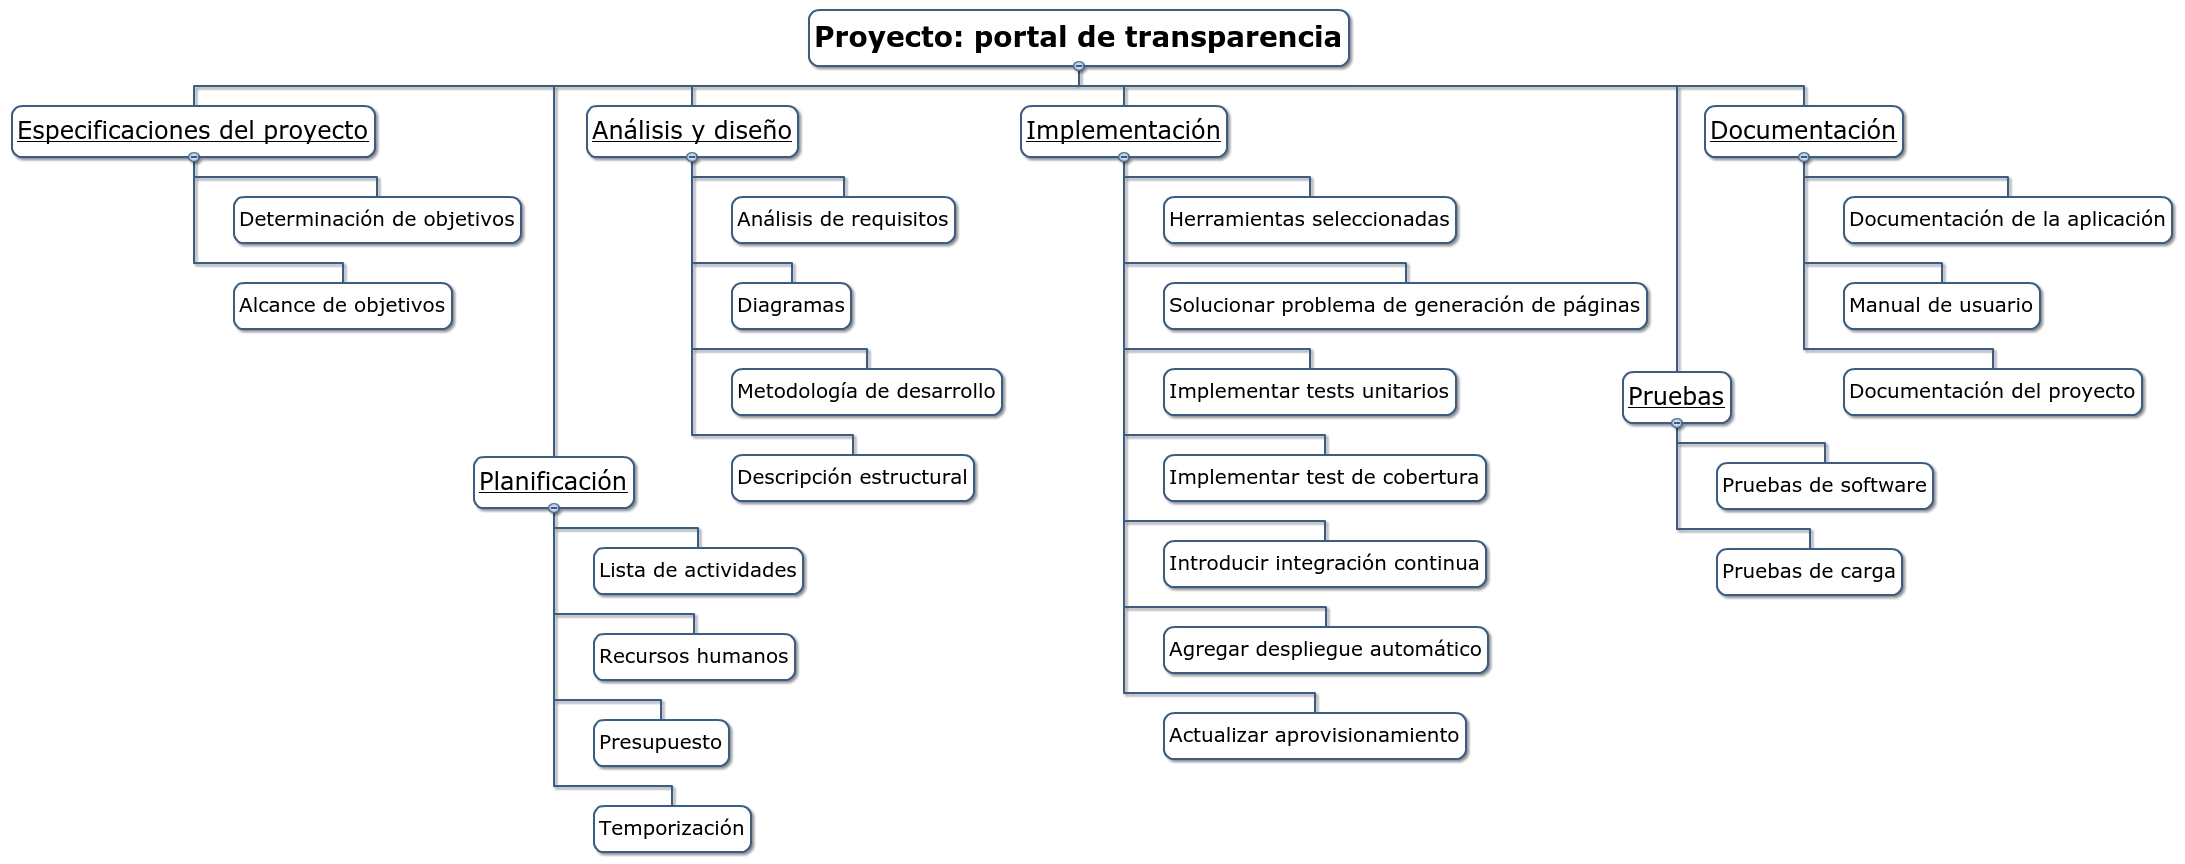
\includegraphics[scale=0.25,angle=90]{imagenes/diagrama_edt.png}
    \caption{Diagrama de Estructura de Descomposición de Trabajo}
    \label{fig:diag_edt}
  \end{center}
\end{figure}

\newpage
\begin{figure}[!ht]
  \begin{center}
    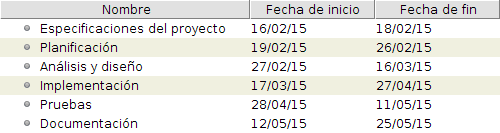
\includegraphics[width=1\textwidth]{imagenes/tempo_tareas.png}
    \caption{Temporización de las tareas}
    \label{fig:tempo_tareas}
  \end{center}
\end{figure}

% \begin{table}[!ht]
%   \begin{center}
%     \begin{tabular}{|l|l|l|}
%       \hline
%       \multicolumn{1}{|c|}{{\bf Nombre}} & \multicolumn{1}{c|}{{\bf Fecha de inicio}} & \multicolumn{1}{c|}{{\bf Fecha de fin}} \\ \hline
%       Especificaciones del proyecto      & 16/02/15                                   & 18/02/15                                \\ \hline
%       Planificación                      & 19/02/15                                   & 26/02/15                                \\ \hline
%       Análisis y diseño                  & 27/02/15                                   & 16/03/15                                \\ \hline
%       Implementación                     & 17/03/15                                   & 27/04/15                                \\ \hline
%       Pruebas                            & 28/04/15                                   & 11/05/15                                \\ \hline
%       Documentación                      & 12/05/15                                   & 25/05/15                                \\ \hline
%     \end{tabular}
%     \caption{Temporización de las tareas}
%     \label{table:tempo_tareas}
%   \end{center}
% \end{table}

\begin{figure}[!ht]
  \begin{center}
    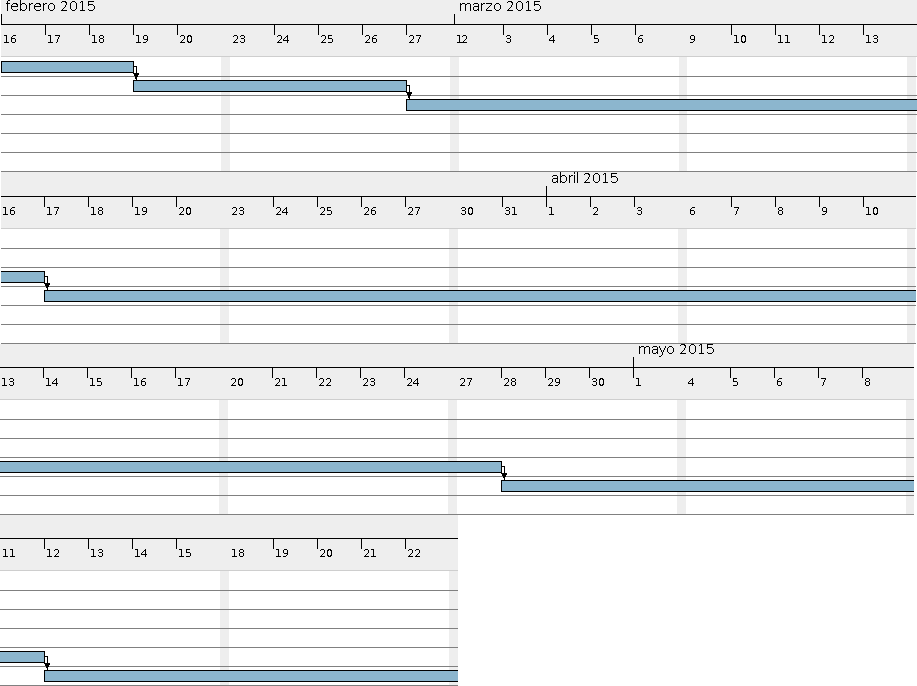
\includegraphics[width=1\textwidth]{imagenes/diagrama_gantt.png}
    \caption{Diagrama de Gantt}
    \label{fig:diag_edt}
  \end{center}
\end{figure}
  \chapter{Análisis y diseño}

\section{Análisis de requisitos}

Todo software se desarrolla para cubrir una necesidad, por lo que en este apartado vamos a describir los requisitos que se 
estiman necesarios para cubrir los objetivos propuestos.

\subsection{Descripción de los actores}

El usuario de la aplicación será cualquier persona que tenga interés por conocer datos internos de la Universidad de Granada 
fácilmente. Como no se quiere enfocar en un público objetivo, el portal tiene que ser fácil de utilizar tanto para personas 
con experiencia en la navegación de páginas web como para las que no la tengan.

\bigskip
También tenemos al desarrollador, que será el encargado de introducir los elementos de información que serán listado en la
plataforma. Como es una página estática, los elementos serán mostados en la tabla correspondiente de la página correspondiente
después de que sean leidos del archivo JSON correspondiente.

\subsection{Requisitos Funcionales}

Los requisitos funcionales son las características que tiene que implementar el sistema para cubrir todas las necesidades de 
los distintos usuarios. Al usuario lo único que le interesa es ver una página web estática con la información que desea 
consultar, por lo que el único requisito imprescindible es que cuando pulse una categoría esta se despliegue y cuando se 
pulse un enlace a OpenData UGR este nos lleve al conjunto de datos correspondiente. Además, se habilitará un buscador para que
también se pueda acceder a la información mediante la introducción de palabras clave. 

\newpage
Todos los requisitos funcionales que tratará este proyecto están únicamente dirigidos a la plataforma UGR Transparente.

\begin{itemize}
  \item \textbf{RF-1.} Introducción de nuevos elementos de información.
\end{itemize}

\begin{itemize}
  \item \textbf{RF-2.} Acceso a la información:
  \begin{itemize}
    \item \textbf{RF-2.1.} Al seleccionar una categoría esta se despliega y aparecen sus subcategorías.
    \item \textbf{RF-2.2.} Al seleccionar una subcategoría se muestran todos sus elementos.
    \item \textbf{RF-2.2.} Cuando se pulsa sobre el enlace de un elemento, automáticamente se accede a la información contenida 
    de ese elemento en OpenData UGR.
    \item \textbf{RF-2.3.} Para obtener información sobre un tema en concreto se introducirá el termino clave relacionado en 
    el buscador.
    \end{itemize}
\end{itemize}

\begin{itemize}
  \item \textbf{RF-3.} Presentación de la información:
  \begin{itemize}
    \item \textbf{RF-.1.} Generar tablas con los elementos de información.
    \item \textbf{RF-3.1.} Si el elemento de información no es un archivo PDF este se podrá previsualizar desde el mismo portal
    de transparencia sin necesidad de acceder a OpenData UGR.
    \item \textbf{RF-3.2.} Siempre se podrá descargar el archivo con la información contenido en OpenData UGR sobre cualquier 
    elemento listado.
  \end{itemize}
\end{itemize}
	
Los aspectos de funcionalidad ya se encuentran implementados en su mayoría (solo existen problemas al cargar la información) de
una fase previa al proyecto por lo que esta será la base de la que se partirá para el desarrollo.

\subsection{Requisitos no Funcionales}

Los requisitos no funcionales son las características propias del desarrollo, pero que no tienen que estar relacionadas con su 
funcionalidad. En este caso nos referimos a todas las características que se requieren para que la aplicación siga un 
desarrollo ágil de despliegue continuo y administración automatica de la plataforma UGR Transparente.

\begin{itemize}
  \item \textbf{RN-1.} Procesar la información que será mostrada en las distintas páginas del portal.
  \item \textbf{RN-2.} Implementar tests unitarios para validar que todas las funcionalidades programadas funcionan 
  correctamente.
  \item \textbf{RN-3.} Realizar test de cobertura que compruebe la fiabilidad que proporcionan los tests unitarios.
  \item \textbf{RN-4.} Usar integración continua para asegurarse que los cambios introducidos no producen conflictos en la 
  plataforma.
  \item \textbf{RN-5.} Usar despliegue automático para actualizar con los nuevos cambios la plataforma una vez estos han sido 
  validados.
  \item \textbf{RN-6.} Elaborar una aprovisionamiento que permita que en una infraestructura por determinar se pueda instalar 
  automáticamente la plataforma y todos los elementos necesarios.
\end{itemize}

En cuanto a la plataforma OpenData UGR, este proyecto solo contempla un único objetivo no funcional que está relacionado con
la administración del sistema más que con que aspectos de desarrollo software.

\begin{itemize}
  \item \textbf{RN-7.} Crear una aprovisionamiento y personalización de CKAN para OpenData UGR.
\end{itemize}

\subsection{Requisitos de Información}

Los requisitos de información se refieren a la información que es necesaria almacenar en el sistema. La única información 
relevante que se va a almacenar son los datos descriptivos y de enlace de cada uno de los elementos del portal OpenData UGR 
que se van a mostrar en UGR Transparente.

\begin{itemize}
  \item \textbf{RI-1.} Datos abiertos.
  \begin{itemize}
    \item Información sobre cada uno de los elementos que se van a mostrar en el portal de transparencia como datos abiertos.
    \item Contenido: nombre, categoría, conjunto de datos, enlace a OpenData UGR, enlace al recurso.
  \end{itemize}
\end{itemize}

\section{Modelos de casos de uso}

Aunque ya se ha indicado que la parte funcional ya se encuentra implementada de forma previa a este proyecto, se van a incluir
unos modelos de caso de uso simples para dar un visión más clara del funcionamiento general de la plataforma UGR Transparente.

\newpage
\subsection{Descripción básica de actores}

\begin{itemize}
  \item \textbf{Ac-1.} Usuario
  \begin{itemize}
   \item Descripción: Persona que usa la plataforma que consulta datos.
   \item Características: Es el usuario común que accederá a la página.
   \item Relaciones: Ninguna.
   \item Atributos: Ninguno.
   \item Comentarios: El usuario no es necesario que tenga ningún conocimiento previo al uso de la plataforma, simplemente
   accederá y consultará los datos que sean de su interes.
  \end{itemize}
  
  \item \textbf{Ac-1.} Desarrollador
  \begin{itemize}
   \item Descripción: Encargado de añadir los elementos de información a la plataforma.
   \item Características: Su trabajo está en el lado del servidor que genera la página, nunca trabaja desde el lado del cliente.
   \item Relaciones: Ninguna.
   \item Atributos: Ninguno.
   \item Comentarios: Es el encargado de desarrollar las funcionalidades del portal, entre ellas añadir nuevos elementos de
   información.
  \end{itemize}
\end{itemize}

\subsection{Descripción casos de uso}

\begin{itemize}
 \item \textbf{CU-1.} Añadir elemento
 \begin{itemize}
  \item Actores: Desarrollador
  \item Tipo: Primario, Esencial
  \item Precondición: Ninguna
  \item Postcondición: Nuevos elementos de información serán visualizados en el portal de transparencia
  \item Propósito: Son añadidos nuevos elementos de información al portal de transparencia.
  \item Resumen: Aparecerán nuevos elementos de informaciónen la categória que corresponda, acompañado además de su enlace
  correspondiente al OpenData UGR, un botón para previsualizar la información y otro botón para descargar el elemento.
 \end{itemize}
\end{itemize}

\newpage
\begin{itemize}
 \item \textbf{CU-2.} Consultar elementos
 \begin{itemize}
  \item Actores: Usuario
  \item Tipo: Primario, esencial
  \item Precondición: Existan elementos de información.
  \item Postcondición: Se muestran los elementos de información de un determinado conjunto de datos.
  \item Propósito: Obtiene los elementos de información de un determinado conjunto de datos.
  \item Resumen: Accediendo a través del panel principal o el buscador se obtiene una tabla con los elementos de información
  de un determinado conjunto de datos.
 \end{itemize}
\end{itemize}

\begin{itemize}
 \item \textbf{CU-3.} Acceder enlace de elemento
 \begin{itemize}
  \item Actores: Usuario
  \item Tipo: Primario, esencial
  \item Precondición: Se hayan generado las tablas con los elementos de información.
  \item Postcondición: 
  \item Propósito: Accede a la información del elemento contenida en OpenData UGR.
  \item Resumen: Cuando se pulsa el enlace, se accede al conjunto de datos que contiene la información del elemento en OpenData
  UGR, presentándolo de distinta forma en función del formato del elemento y dando la opción de descagar ese mismo elemento en 
  un archivo con su formato original.
 \end{itemize}
\end{itemize}

\begin{itemize}
 \item \textbf{CU-4.} Previsualizar elemento de información
 \begin{itemize}
  \item Actores: Usuario
  \item Tipo: Secundario
  \item Precondición: Se hayan generado las tablas con los elementos de información.
  \item Postcondición: 
  \item Propósito: Previsualiza los datos del elemento.
  \item Resumen: Cuando se selecciona el botón de ver un elemento de la tabla se abre una ventana emergente en la que se 
  muestra la información del elemento que se contiene en OpenData UGR.
 \end{itemize}
\end{itemize}

\newpage
\begin{itemize}
 \item \textbf{CU-5.} Descargar elemento de información
 \begin{itemize}
  \item Actores: Usuario
  \item Tipo: Secundario
  \item Precondición: Se hayan generado las tablas con los elementos de información.
  \item Postcondición: 
  \item Propósito: Descagar el elemento en un archivo con su formato original.
  \item Resumen: Cuando se selecciona el botón de descargar un elemento de la tabla se abre una ventana emergente en la que se
  muestra la información del elemento que se contiene en OpenData UGR.
 \end{itemize}
\end{itemize}

\subsection{Diagramas de casos de uso}

Desde un punto de vista funcional es el usuario el que realiza la mayoria de las acciones del portal, la función del 
desarrollar aunque fundamental, solo es una acción que se realiza en un segundo plano del que no se tiene constancia desde 
fuera.

\begin{figure}[!h]
  \begin{center}
  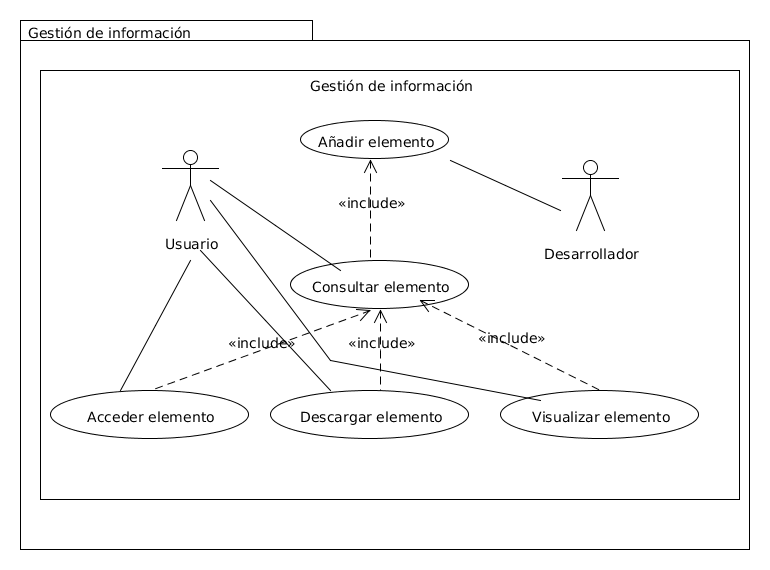
\includegraphics[width=1\textwidth]{imagenes/diagrama_casos_uso.png}
  \caption[Casos de uso]{Diagrama de casos de uso}
  \label{fig:casosUso}
  \end{center}
\end{figure}


  \chapter{Implementación}
  %\input{capitulos/06_Pruebas}
  %\input{capitulos/07_Conclusiones y Trabajos Futuros}
% \backmatter
%%\nocite{*}
%\bibliography{bibliografia/bibliografia}\addcontentsline{toc}{chapter}{Bibliografía}
%\bibliographystyle{miunsrturl}
%
%\appendix
%\input{apendices/manual_usuario/manual_usuario}
%\input{glosario/entradas_glosario}
%\addcontentsline{toc}{chapter}{Glosario}
%\printglossary

\newpage
\thispagestyle{empty}
\
\end{document}